\chapter{Marco teórico}
\label{ch:marco}

En

\section{Péndulo amortiguado a hélice (PAMH)}

El péndulo amortiguado a hélice corresponde a una planta de laboratorio compuesta de un motor con hélice controlado por torque, una masa pequeña, péndulo y soportes de aluminio de baja fricción. Un modelo simplificado del sistema se muestra en la Figura \ref{fig:modpen} \textcolor{SkyBlue}{PAMH1}.

\begin{figure}[h]
	\centering
	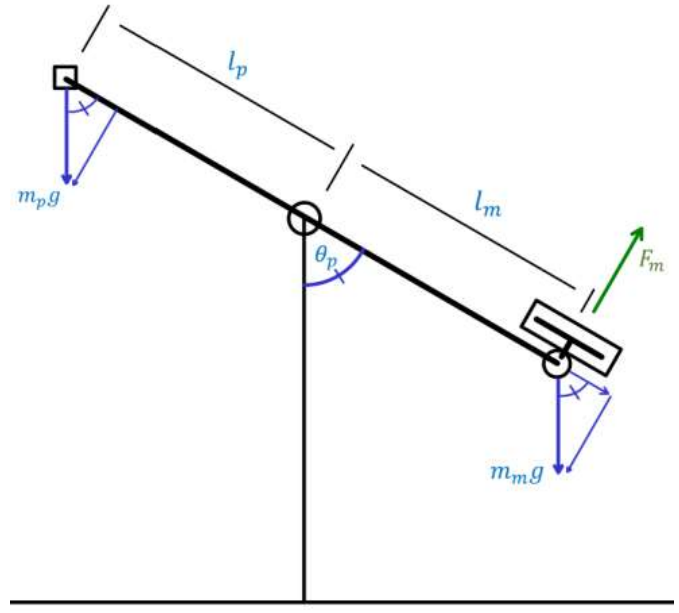
\includegraphics[scale=0.3]{fig/new/ModeloPendulo.png}
	\caption{Modelo simplificado del PAMH.}
	\label{fig:modpen}
\end{figure}

El objetivo de dicho sistema es controlar la magnitud del ángulo $\theta_p$, únicamente ejerciendo torque al accionar a una distancia $l_m$ el motor con una fuerza $F_m$ y movimiento de su masa $m_m$, mientras a una distancia de $l_p$ del centro se encuentra una masa $m_p$ que contrarresta el movimiento.

De manera que al analizar el sistema con sumatoria de torques se obtiene la constante de rosamiento central $B$ (en caso de existir) junto con la inercia ejercida $J_p$. Por lo tanto, se definen las variables de estado siguientes y sus ecuaciones de estado mostradas en \ref{ecu:ecuestados} \textcolor{SkyBlue}{ControlModerno}.

\[x_1 = \theta_p \qquad x_2 = \dot{\theta}_p \qquad y = x_1 = \theta_p\]
\begin{equation}
	\left \{ \begin{array}{lcc} \dot{x}_1 = x_2 \\ \\ \dot{x}_2 = -\dfrac{B}{J_p} x_2 + (m_p l_p -m_m l_m)\dfrac{g}{J_p}sen(x_1) +\dfrac{l_m}{J_p}F_m \end{array} \right.
	\label{ecu:ecuestados}
\end{equation}




\section{Aprendizaje reforzado (RL)}


Al estudiar el concepto de aprendizaje reforzado y los diferentes métodos y algoritmos que corresponden a este tipo de aprendizaje automático, se obtiene el resumen de la Figura \ref{fig:teoriaRL}, en donde se muestra que las principales secciones son el RL basado en modelo y el libre de modelo. De igual forma se cuenta con el aprendizaje reforzado profundo (DRL), una combinación y reestructuración de métodos de cada subdivisión \textcolor{SkyBlue}{DataScience}.

\begin{figure}[hh]
	\centering
	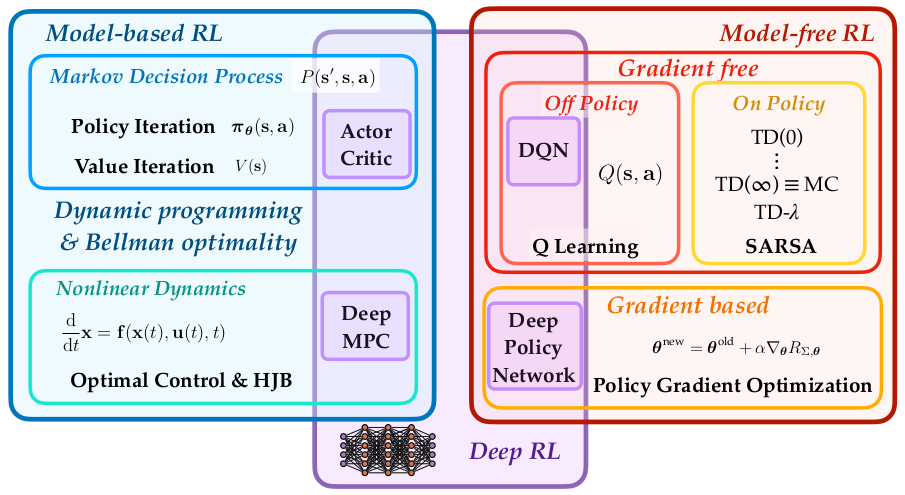
\includegraphics[scale=0.35]{fig/new/CatRL.png}
	\caption{Resumen de categorización del RL \textcolor{SkyBlue}{DataScience}.}
	\label{fig:teoriaRL}
\end{figure}


De igual manera, los avances en la investigación de diferentes métodos como las redes neuronales recurrentes (RNN), ejemplificado por Mamba \textcolor{SkyBlue}{Mamba}, ha mostrado la capacidad de optimización del desempeño de estas para llegar a competir con los modelos basados en \textit{Transformer}.


\begin{comment}


%References

@article{PAMH1,
author = {Castaño Hernández, A. and Moreno Beltrán, J. P. and Hernández Pérez, J. F. and Villafuerte Segura, R.},
year = {2018},
title = {Diseño y control de un sistema balancín con motor y hélice de bajo costo},
journal = {ICBI},
volume = {5},
numbre = {10},
doi = {https://doi.org/10.29057/icbi.v5i10.2937}
}

@article{Mamba,
author = {Gu, Albert and Dao, Tri},
year = {2023},
title = {Mamba: Linear-Time Sequence Modeling with Selective State Spaces},
journal = {Cornell University, Arxiv},
doi = {https://doi.org/10.48550/arXiv.2312.00752}
}

\end{comment}



\subsection{DQN}

DQN es un algoritmo de aprendizaje por refuerzo basado en valores introducido por DeepMind en 2013. Se diseñó específicamente para aprender a jugar a juegos de Atari directamente a partir de entradas de píxeles sin procesar3. Estos son los aspectos clave de DQN:

Q-Learning y Diferencia Temporal:
La "Q" en DQN significa "Q-Learning", que es un método de diferencia temporal fuera de política.
DQN tiene en cuenta las recompensas futuras al actualizar la función de valor para un par estado-acción determinado.
A diferencia de los métodos de gradiente de política (por ejemplo, REINFORCE), DQN no requiere esperar hasta el final de un episodio para calcular la recompensa final.
Atari Games y Raw Pixels:
DQN ganó popularidad al aprender con éxito a jugar a juegos de Atari utilizando datos de píxeles en bruto como entrada.
El agente aprende a realizar acciones basándose en los valores de píxeles observados, sin ninguna característica creada a mano.
La ecuación de Bellman guía las actualizaciones de la función de valor a medida que el agente interactúa con el entorno.
Ejemplo de MountainCar-v0:
Consideremos el entorno MountainCar-v0 de OpenAI Gym.
En esta tarea, un coche con poca potencia debe subir una colina empinada cogiendo suficiente impulso.
El agente recibe una recompensa de -1 por cada acción realizada hasta que alcanza la bandera (recompensa 0).
El episodio termina si el agente no consigue alcanzar la montaña en 200 pasos.



\subsection{PPO}



Función objetivo:
PPO utiliza una función objetivo sustituta para restringir el tamaño del paso durante las actualizaciones de la política. Esto garantiza un aprendizaje estable y eficaz.
A diferencia de otros algoritmos, PPO no requiere esperar hasta el final de un episodio para calcular la recompensa final, sino que actualiza la función de valor de forma incremental a medida que el agente interactúa con el entorno.
Estimación de ventaja generalizada (GAE):
Aunque el documento original de la PPO hace abstracción de la estimación de ventajas en su objetivo, la aplicación real utiliza GAE.
GAE ayuda a estimar las ventajas de diferentes acciones basándose en las recompensas y funciones de valor observadas.
Normalización de ventajas:
Después de calcular las ventajas utilizando GAE, PPO normaliza las ventajas restando la media y dividiendo por la desviación estándar.
Cabe destacar que esta normalización se produce a nivel de minilotes, no a nivel de lotes completos2.


AAAA \cite{PPO2017}







\section{Métricas de evaluación}

Función de recompensa: Especificar la señal de recompensa (por ejemplo, minimizar el consumo de energía, estabilizar el péndulo).

Criterios de convergencia: Describa cuándo se considera que el algoritmo ha tenido éxito.
